\documentclass[times, utf8, zavrsni]{fer}
\usepackage{booktabs}
\usepackage[hyphenbreaks]{breakurl}
\usepackage{gensymb}

\begin{document}

\thesisnumber{7031}

\title{Višedretvena izvedba algoritma računanja histograma orijentacija gradijenata u slikama}

\author{Mateo Imbrišak}

\maketitle

% Dodavanje zahvale ili prazne stranice. Ako ne želite dodati zahvalu, naredbu ostavite radi prazne stranice.
\zahvala{}

\tableofcontents

\chapter{Uvod}
Uporaba računalnog vida je danas jako raširena. Koristi se u sustavima za raspoznavanje objekata na slikama, prepoznavanje osoba, prebrojavanje pojedinih objekata na slici te kao pomoć pri orijentaciji autonomnih vozila. U svim područjima je poželjna veća brzina izvođenja no u nekima je upravo to ključna značajka. Glavni problem brzini izvođenja predstavlja činjenica da je proces dobivanje računalu korisnih podataka iz slike računski vrlo zahtjevan. Veliki broj modernih algoritama računalnog vida često izvodi identične i nezavisne operacije na velikom broju piksela pojedine slike te ih je zato moguće značajno ubrzati višedretvenom izvedbom. \\

Cilj ovog rada je ostvariti višedretvenu izvedbu algoritma računanja opisnika temeljenog na histogramu orijentacija gradijenata pomoću kojeg je moguće naučiti neki model da raspoznaje sadrži li neka slika traženi objekt ili ne. Iako se navedeni postupak može koristiti za detekciju proizvoljnih objekata u ovom radu koristi se prozor širine 64 i visine 128 pikseal, kao i u originalnom radu \citep{dalal2005histograms}, predviđen za detekciju pješaka. \\

Osnovni pojmovi, provlemi i prednosti višedretvenosti detaljnije se objašnjeni u drugom poglavlju. Treće poglavlje opisuje postupak računanja histograma orijentacija gradijenata u slikama. Opis detekcije objekata kao i model koji se koristi u te svrhe opisani su u četvrtom poglavlju. Peto poglavlje opisuje implementaciju programskog rješenja dok šesto analizira rezultate i performanse implementacije. Na kraju se nalazi zaključak te je dan popis korištene literature kao i sažetak na hrvatskom i negleskom jeziku.

\chapter{Višedretvena paralelizacija}
Gotovo sva računala danas koriste višejezgrene procesore što omogućava paralelno izvođenje više dretvi i tako je moguće postiči značajno ubrzanje izvođenja nekog posla, ako za taj posao nije potrebno pisati rezultate u zajedničke varijable. Upravo se taj pristup koristi kako bi se ostvarial paralelizacija u ovom radu.

\section{Dretva}
Dretva je definirana kao niz instrukcija koje slijedno izvodi jezgra procesora. Svaka dretva ima svoje resurse koje može koristiti. Računalo može pokrenuti više dretvi nego što ima dostupnih jezgri procesora, no broj jezgri ograničava maksimalan broj dretvi koji se može izvoditi paralelno. Ako je istovremeno pokrenuto više dretvi nego što je dostupno jezgri procesora one će se i dalje sve izvoditi, ali ne uvijek istovremeno već će se izmjenjivati što dovodi do čestoih promjena konteksta \citep{os}.

\section{Promjene konteksta}
Promjena konteksta \engl{context switching} nastupa kada dolazi do promjene aktivne dretve. Kao što je već rečeno svaka dretva koristi svoje resurse i u aktivnom stanju raspolaže registrima na procesoru. Kada dretva prestaje biti aktivna, ali još nije obavila cijeli posao, potrebno je u memoriju spremiti trenutni kontekst te dretve kako bi se mogao ponovno koristiti kada dretva postane aktivna. Nakon toga je potrebno učitati kontekst dretve koja sada postaje aktivna. Te operacije imaju određeno trajanje te nije poželjno raditi promjenu konteksta češće nego što je to potrebno, odnosno nije poželjno paliti više dretvi istovremeno ako ih nije moguće paralelno izvoditi jer se tako smanjuje efikasnost obavljanja posla \citep{os}. Slika~\ref{fig:contextSwitching} prikazuje promjenu konteksta gdje dretva \textit{thread1} prestaje biti aktivna, a dretva \textit{thread2} postaje aktivna.

\begin{figure}[htb]
	\centering
	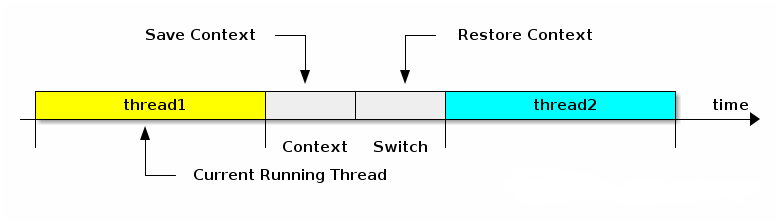
\includegraphics[width=\linewidth]{figures/contextSwitching.png}
	\caption{Promjena konteksta\protect\footnotemark}
	\label{fig:contextSwitching}
\end{figure}

\def\UrlBreaks{\do\/\do-}
\footnotetext{Izvor: \burl{https://developpaper.com/understanding-system-structure-from-java-perspective-1-cpu-context-switch/}}

\section{Kritični odsječak}
Dretve mogu koristiti neke zajedničke resurse. Moguće je istovremeno čitanje zajedničkih resursa, no ako je potrebno promijeniti vrijednost neke varijable moguće je da dvije ili više dretvi to pokušaju učiniti istovremeno. Kako se promjena jedne dretve nebi izgubila istovremenim pisanjem druge dretve potrebno je osigurati da samo jedna dretva u bilo kojem trenutku može modificirati tu vrijednost. Dio posla koji smije obavljati samo jedna dretva u bilo kojem trenutku naziva se kritični odsječak \engl{critical section}. Kako bi se kritični odsječak zaštitio koriste se sinkronizacijski mehanizmi. U ovom radu korištene su blokirajuće strukture podataka. Kada dretva pokuša koristiti blokirajuću strukturu podataka koju već koristi neka druga dretva ona postaje blokirana, odnosno mora čekati da prva dretva prestane koristiti tu strukturu podataka i tek tada može nastaviti svoje izvođenje \citep{os}.

\chapter{Algoritam računanja histograma orijentacija gradijenata u slikama}
Algoritam računanja histograma orijentacija gradijenata \engl{histogram of oriented gradients} koristi se kako bi se za sliku izračunao njezin opisnik koji sadrži sažete, korisne informacije o toj slici. Dobiveni opisnik može se proslijediti nekom naučenom klasifikatoru koji na temelju njega može odrediti sadrži li slika (ili obrađeni dio slike) traženi objekt. Izračun opisnika se provodi na dijelu slike određene veličine, a točne dimenzije dijela slike koji se koristi ovise o traženom objektu. Glavna ideja je da se traženi objekt može prepoznati pomoću njegovih bridova i orijentacije tih bridova te se zato koristi gradijent.

\section{Izračun gradijenta}
Prije samog izračuna gradijenta moguće je normalizirati boje i gama vrijednosti, ali kako je u originalnom radu \citep{dalal2005histograms} pokazano da to ne utječe značajno na rezultate zbog kasnije normalizacije opisnika, u ovom radu je taj korak preskočen. Za izračun gradijenta sliku je potrebno filtrirati određenom maskom u smjeru \(x\)-osi i \(y\)-osi. U originalnom radu \citep{dalal2005histograms} isprobano je nekoliko tipova maski no najbolja se pokazala jednostavna 1-D centrirana maska koja se zato koristi i u ovom radu: 

\begin{equation}
	[-1, 0, 1]
	\label{eq:mask}
\end{equation}

Uz korištenje maske u formuli \ref{eq:mask} za pojedini piksel \(I\) potrebno je izračunati derivaciju u smjeru \(x\) i \(y\)-osi prema formulama:

\begin{equation}
I_x(r, c) = I(r, c + 1) - I(r, c - 1)
\label{eq:dx}
\end{equation}

\begin{equation}
I_y(r, c) = I(r - 1, c) - I(r + 1, c)
\label{eq:dy}
\end{equation}

U formulama \ref{eq:dx} i \ref{eq:dy} \(r\) predstavlja redak slike, a \(c\) predstavlja stupac slike \citep{tomasi2012histograms}. Ako slika sadrži više boja odnosno kanala, postupak se ponavlja za svaki kanal. Na temelju dobivenih derivacija potrebno je izračunati magnitudu i kut koji će se koristiti u kasnijim koracima:

\begin{equation}
\mu = \sqrt{I_x^2 + I_y^2}
\label{eq:mag}
\end{equation}

\begin{equation}
\theta = \frac{180}{\pi}(\tan_2^{-1}(I_y, I_x) \mod \pi)
\label{eq:ang}
\end{equation}

Kod detekcije pješaka u radu \cite{dalal2005histograms} pokazalo se najbolje koristiti kuteve između 0\degree i 180\degree, odnosno kutevi bez orijentacije, no za neke druge probleme kao što je detekcija automobila pokazalo se bolje koristiti kuteve do 360\degree \citep{dalal2005histograms}. U originalnom radu za doprinos magnitude koristi se magnituda kanala koji ima najveću magnitudu, no u ovom radu koristi se doprinos magnituda svih kanala.

\section{Izračun histograma}
Za izračun histograma prvo treba sliku podijeliti u kvadratne ili kružne čelije koje se međusobno ne preklapaju. U ovom radu se koriste kvadratne čelije širine 8 piksela i visine 8 piksela. Slika~\ref{fig:hogCells} prikazuje uvećanu sliku dimenzija 64 na 128 piksela podijeljenu u čelije dimenzija 8 na 8 piksela.

\begin{figure}[htb]
	\centering
	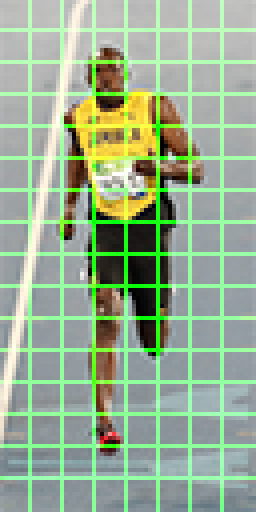
\includegraphics[width=0.3\linewidth]{figures/hog-cells.png}
	\caption{Slika podijeljena u čelije\protect\footnotemark}
	\label{fig:hogCells}
\end{figure}

\footnotetext{Izvor: \burl{https://www.learnopencv.com/histogram-of-oriented-gradients/}}


Za svaku čeliju zatim se računa histogram orijentacije gradijenata. U radu \citep{dalal2005histograms} pokazalo se da za detekciju pješaka preciznost rase s povećanjem broja stupaca po histogramu do broja 9 te se zato i u ovom radu koristi upravo devet stupaca. Raspon svakog stupca definiran je formulom:

\begin{equation}
	w = \frac{180}{B}
	\label{eq:width}
\end{equation}

U formuli \ref{eq:width} \(B\) predstavlja broj stupaca \citep{tomasi2012histograms}. Potrebno je izračunati doprinos magnitude za svaki piksel unutar pojedine čelije. Za izračun doprinosa potrebno jedefinirati sredinu raspona pojedinog stupca formulom:

\begin{equation}
	c_i = w(i + \frac{1}{2})
	\label{eq:center}
\end{equation}

 U formuli \ref{eq:center} \(w\) predstavlja širinu stupca, a \(i\) indeks stupca. Piksel svojom magnitudom doprinosi stupcu kojem pripada po some kutu i slijedećem stupcu ovisno o udaljenosti kuta od središta stupca kojem pripada, a to je prikazano formulama: 
 
 \begin{equation}
	v_{j} = \mu \frac{c_{j + 1} - \theta}{w}
 	\label{eq:vote}
 \end{equation}
 
 \begin{equation}
 	v_{j+1} = \mu \frac{\theta - c_j}{w}
 	\label{eq:voteNext}
\end{equation}

Zbroj vrijednosti iz formula \ref{eq:vote} i \ref{eq:voteNext} mora biti \(\mu\) jer piksel vrijednosti stupca doprinosi cijelom svojom magnitudom \citep{tomasi2012histograms}. Slika~\ref{fig:vote} prikazuje podjelu doprinosa magnitude \(\mu \) uz kut od 77\degree i devet stupaca po čeliji. Doprinos stupcu histograma može biti sama vrijednost magnitude, ali može biti i neka druga vrijednost kao kvadrat ili korijen magnitude. U radu \cite{dalal2005histograms} ustanovilo se da se u praksi najbolji rezultati dobiju ako se koristi vrijednost magnitude te je zato ta vrijednost korištena i u ovom radu.

\begin{figure}[htb]
	\centering
	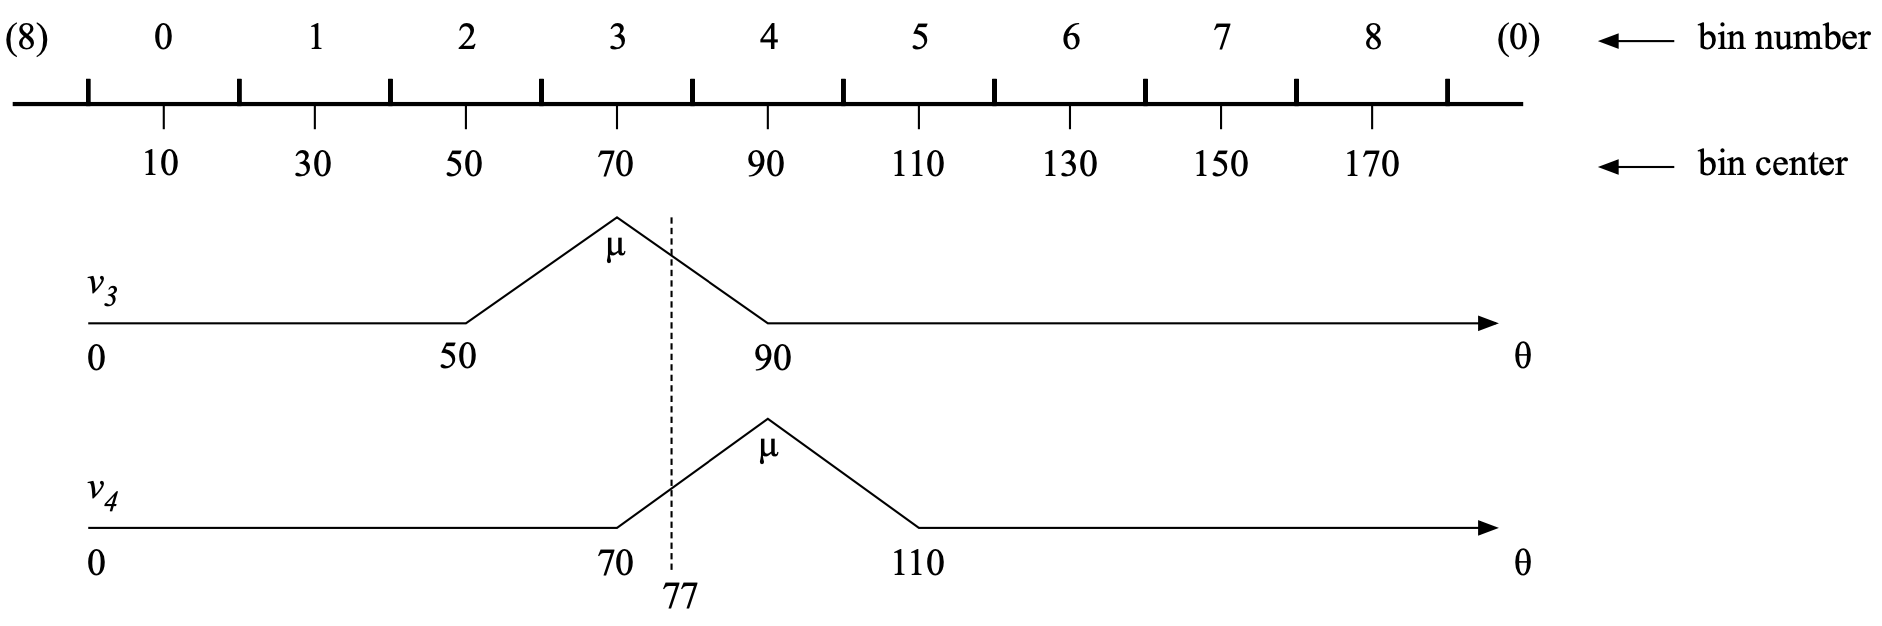
\includegraphics[width=\linewidth]{figures/vote.png}
	\caption{Slika podijeljena u čelije\protect\footnotemark}
	\label{fig:vote}
\end{figure}

\footnotetext{Izvor: \citep{tomasi2012histograms}}

\section{Normalizacija blokova}
Lokalno osvjetljenje i kontrast mogu znatno utjecati na magnitudu gradijenta. Iz tog razloga vrlo je važno normalizirati blokove susjednih čelija. Odabrani su blokovi širine 4 i visine 4 čelije. U radu \cite{dalal2005histograms} ustanovljeno je da preklapanje blokova na pola bloka pozitvino utjeće na preciznost detekcije tako da je u ovom radu za pomak bloka korištena jedna čelija. Vrijednosti u bloku zapisane u obliku vektora normiraju se formulom:

\begin{equation}
	v = \frac{v}{\sqrt{\left\|v\right\|^2 + \epsilon}}
	\label{eq:norm}
\end{equation}

Vrijednost $\epsilon$ u formuli \ref{eq:norm} predstavlja malu pozitivnu konstantu kako bi se izbjeglo potencijalno dijeljenje s nulom \citep{tomasi2012histograms}.

\section{Normalizacija opisnika}

\chapter{Detekcija pješaka}

\chapter{Programsko rješenje}

\chapter{Rezultati}

\chapter{Zaključak}
Zaključak.

\bibliography{literatura}
\bibliographystyle{fer}

\begin{sazetak}
Sažetak na hrvatskom jeziku.

\kljucnerijeci{Ključne riječi, odvojene zarezima.}
\end{sazetak}

\engtitle{Multi-threaded Implementation of Algorithm for Calculation of Histogram of Oriented Gradients in Images}
\begin{abstract}
Abstract.

\keywords{Keywords.}
\end{abstract}

\end{document}
